% /* cSpell:enable */
% /* cSpell:locale de,en */
\chapter{Einleitung}
\label{cha:Einleitung}

Seit Anfang 2020 beschäftigt uns nun COVID-19. Die Pandemie hat nicht nur zahlreiche Forschungsgebiete bewegt, sondern auch viele gesellschaftliche Fragen aufgeworfen. Von Beginn an standen Fragen wie "Welche Maßnahmen sind wirkungsvoll?" und "Auf welche Einschränkungen kann man verzichten?" im Diskussionsmittelpunkt. Dies betraf nicht nur die Forschung, sondern war immer auch ein Thema mit gesellschaftlicher Verantwortung. Sind Ausgehbeschränkungen notwendig, oder reicht es aus, Abstand zu halten? Ist die Ansteckungsgefahr in Schulen höher als in Büros? Welche Reisen sind weiterhin notwendig und unter welchen Voraussetzungen sollen diese möglich sein? Auf welche Dienstleistungen und Freizeitangebote können wir verzichten?
Diese Frage wird natürlich sehr individuell unterschiedlich beantwortet, deshalb ist es wichtig, einen gemeinschaftlichen Konsens zu finden.

Mit dem Aufkommen der Impfung hat sich dann auch die Frage gestellt, welcher Wirkstoff wirksamer ist oder ob überhaupt Impfstoffe wirksam sind. Dies war eng mit der Frage verknüpft, was Wirksamkeit denn eigentlich bedeutet. Bedeutet Wirksamkeit, dass die Ansteckungsgefahr gesenkt wird? Um wie viel muss die Ansteckungsgefahr gesenkt werden? Oder muss ein Impfstoff, um wirksam zu sein, lediglich Krankheitssymptome abmildern? Oder geht es um den Schutz von besonders vulnerablen Menschen? Welche Risiken dürfen hierbei in Kauf genommen werden?

\section{Der Begriff Wirksamkeit}
\label{sec:wirksamkeit}

Das Robert-Koch-Institut unterscheidet zwischen Impfstoffwirksamkeit und Impfstoffeffektivität und definiert diese beiden Begriffe wie folgt: \cite{rki-handbuch}

\begin{description}
    \item[Impfstoffeffektivität] "Die Gesamtauswirkungen des Einsatzes eines Impfstoffs; neben der direkten Impfstoffwirksamkeit können die indirekten Wirkungen der Impfung (wie die Reduktion der Inzidenz, Krankenhausbehandlungen, tödliche Ausgänge der Zielkrankheit) nach breiter Anwendung des Impfstoffs in einer Population unter Alltagsbedingungen in Studien ermittelt werden."

    \item[Impfstoffwirksamkeit] "Als direkte Wirkung des Impfstoffs wird die relative Reduktion des Risikos, nach Impfung im Vergleich zu Nichtgeimpften an der Zielkrankheit zu erkranken, vorzugsweise in kontrollierten Studien unter optimalen Bedingungen ermittelt. Als Maß für die Wirksamkeit eines Impfstoffs (IW) kann das Verhältnis der Erkrankungsquote bei Geimpften (EG) zu der bei Nichtgeimpften (ENG) ermittelt werden:"
    
    $IW(\%) = \frac{ENG-E}{ENG} \times 100$
\end{description}

Trotz dieser Definition sind Diskussionen über die Wirksamkeit neu entbrannt, aber auch über Impfpflichten und persönliche Rechte wurde debattiert.

\section{Krankheit und Virus}
\label{sec:virusinfo}
Die Krankheit COVID-19 wird vom Coronavirus SARS-CoV-2 verursacht. Bis jetzt gibt es zahlreiche Mutationen, die beobachtet werden. Zwei Varianten -- Delta und Omikron -- wurden vom "Centers for Disease Control and Prevention" (CDC) als "besorgniserregend" eingestuft, wobei erstere seit April wieder auf "beobachtet" zurückgestuft wurde. \cite{cdc-classification}
Die Übertragung erfolgt laut Robert Koch-Institut (RKI) vor allem über Respiration, eine Kontaktübertragung ist aber vor allem in unmittelbarer Umgebung infektiöser Personen nicht ausgeschlossen. Die Inkubationszeit beträgt im Median vier bis sechs Tage, häufige Symptome sind unter anderem Husten, Fieber, Schnupfen und Störung des Geruchs- und/oder Geschmackssinnes. Eine hohe Infektiösität besteht bereits vor dem Auftreten von Symptomen. Zur Einschränkung der Übertragung werden eine schnelle Isolierung positiver Personen, Identifizierung von Kontaktpersonen sowie Einhaltung von Hygieneregeln, das Tragen von Masken und Lüften empfohlen. Geimpfte Personen können sich prinzipiell infizieren und auch zu Überträgern werden, jedoch mit deutlich verringerter Wahrscheinlichkeit. \cite{rki}
Unter diesen Voraussetzungen ist zu erwarten, dass sowohl die COVID-19-Impfung als auch Einschränkungen von Veranstaltungen oder Ansammlungen sowie Reisebeschränkungen aktiv helfen, sowie diese Maßnahmen durch eine frühe Erkennung der Krankheit durch Tests oder Früherkennungssysteme die Fallzahlen senken.


\section{Verlauf der Pandemie}
\label{sec:pandemieverlauf}

Nach dem Ausbruch im Dezember 2019 wurde von der Weltgesundheitsorganisation WHO am 11. März 2020 die bis dahin als Epidemie eingestufte Krankheit offiziell zur weltweiten Pandemie erklärt. Kurz darauf wurden in Europa Maßnahmen beschlossen, um die weitere Verbreitung einzudämmen. Die im ersten Lockdown noch strengen Maßnahmen wurden im Sommer wieder gelockert, jedoch im Herbst, wenn auch weniger restriktiv, wieder eingeführt.

Im Dezember 2020 kamen zudem erste Impfstoffe auf, die im folgendem Sommer 2021 breit verfügbar waren.

Betrachtet man die Todesfälle (s. Abbildung \ref{fig:deaths}), so ist zu erkennen, dass es drei große Pandemiewellen gab -- von März bis Mai 2020, von Oktober 2020 bis Mai 2021 und von September/Oktober 2021 bis Mai 2022. Dabei kam in der zweiten Welle die Delta-Variante des Sars-CoV-2-Viruses auf, ab Dezember 2021 von der Omikron-Variante, die seither die vorherrschende Variante in Europa ist, verdrängt wurde. Vergleicht man die Todesfälle mit den Fallzahlen, wird deutlich, dass die Sterblichkeit des Virus dadurch abnahm.

\begin{figure}[ht]
    \caption{COVID-19-Fälle pro Million Einwohner seit Pandemiebeginn in Europa \cite{owidcoronavirus}}
    \label{fig:cases}
    \centering
    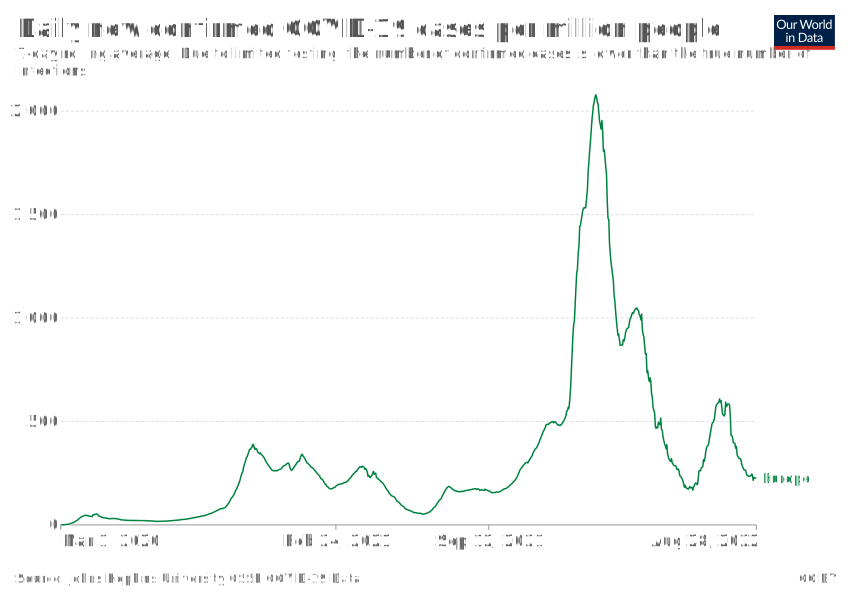
\includegraphics[trim={0 0 0 12cm},clip,width=0.6\linewidth]{coronavirus-data-explorer-europe}
\end{figure}

\begin{figure}[ht]
    \caption{Todesfälle pro Million Einwohner seit Pandemiebeginn in Europa \cite{owidcoronavirus}}
    \label{fig:deaths}
    \centering
    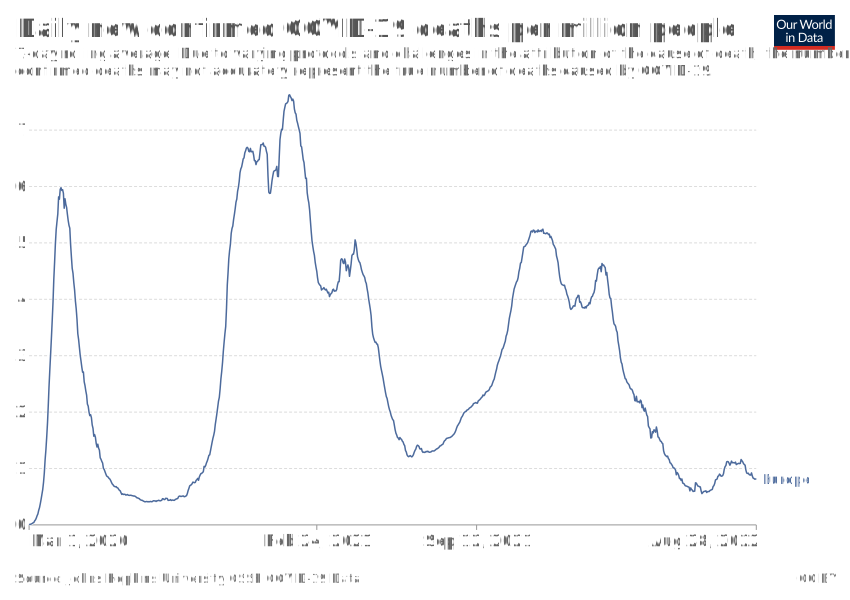
\includegraphics[trim={2cm 0 2cm 12cm},clip,width=0.6\linewidth]{coronavirus-data-explorer-deaths-europe}
\end{figure}

In der folgenden Arbeit werden die Zusammenhänge zwischen Fallzahlen, Maßnahmen und Impfrate untersucht, sowie eine Befragung zum Begriff Wirksamkeit durchgeführt. Die Frage, welche Maßnahmen wirkungsvoll waren und ob sich der Beitrag der Impfrate belegen lässt, sollen beantwortet werden.
% /* cSpell:disable */